\documentclass{article}
\usepackage[utf8x]{inputenc}
\usepackage[russian]{babel}
\usepackage{graphicx}
\usepackage{amsmath}
\usepackage{hyperref}
\usepackage[left=2cm,right=2cm,
    top=2cm,bottom=2cm,bindingoffset=0cm]{geometry}

\begin{document}
\begin{titlepage}
\newpage

\begin{center}

Федеральное государственное автономное образовательное учреждение
высшего образования \\
\large{<<Национальный исследовательский университет} \\
\large{<<Высшая школа экономики>>} \\
Факультет компьютерных наук \\
ООП «Прикладная математика и информатика» \\

\hrulefill
\end{center}

\vspace{8em}

\begin{center}
\huge{Отчёт о прохождении практики \\}
\end{center}

\vspace{20em}
\begin{flushleft}
Студент: Леонов Алексей Олегович \\
Группа: БМПИ161 \\
Вид практики: учебная \\
Руководитель: Авдеев Роман Сергеевич, к.\,ф.-м.\,н., доцент Департамента больших данных и информационного поиска \\
% https://habrahabr.ru/post/207364/
\vspace{0.5cm}
\underline{\hspace{4cm}} \\
\small{(подпись руководителя практики\\ об ознакомлении с отчетом)}
\end{flushleft}


\vspace{\fill}

\begin{center}
Москва, 2017
\end{center}

\end{titlepage}


\tableofcontents

\section{Введение}
Цель практики -- ознакомиться с численными методами решения систем линейных уравнений. Были поставлены следующие задачи:
\begin{enumerate}
    \item Изучение численных методов решения систем линейных уравнений.
    \item Написание соответствующих алгоритмов.
    \item Сравнение их эффективности.
\end{enumerate}

\section{Основная часть:}

\subsection{Изучение и написание алгоритмов}

Для изучения методов потребовалось найти литературу по соответствующей теме. Руководителем практики была предоставлена книга <<Практикум на ЭВМ>> Богачева К.Ю. Кроме того, среди литературы курса <<Численные методы в анализе данных>> на сайте wiki.cs.hse.ru я нашёл учебник <<Лекции по вычислительной математике>> Лобанова А.И. и Петрова И.Б.

Для реализации изученных алгоритмов использовался язык С++. Для построения графиков -- язык Python, библиотека matplotlib.

Ссылка на исходный код программ: \\
\href{https://github.com/alexey9177950/summer-practice}{https://github.com/alexey9177950/summer-practice}

Было реализовано 4 точных (прямых) метода решения систем:
\begin{enumerate}
    \item Метод Гаусса.
    \item Метод Гаусса с выбором главного элемента по столбцу.
    \item Метод Гаусса с выбором главного элемента по всей матрице.
    \item Метод вращений.
\end{enumerate}

И два итерационных: метод простой итерации и метод Зейделя.

\subsection{Описание методов}

Метод Гаусса заключается в приведении матрицы к треугольному виду с помощью элементарных преобразований. При его работе поддерживается инвариант, что после шага с номером $j$ в столбцах расширенной матрицы системы с номерами $k$ ($k \in [1, j]$) $A_{i, k} = 0$ при $i > k$.
На $j$-ом шаге выбирается $i \in \{j, \dots n\} :\ A_{ij} \ne 0$. Это строка меняется местами со строкой номер $j$. Далее $j$-ая строка вычитается из всех с $j+1$ до $n$ с таким коэффициентом, чтобы соответствующие элементы в $j$-ом столбце стали равны нулю.

Отличие метода Гаусса с выбором главного элемента по столбцу заключается в том, что выбирается не просто произвольная строка, где элемент $j$-ого столбца ненулевой, а та, где он максмален по модулю (такой называется главным элементом), так как это обеспечивает наименьшую погрешность.

В ещё одной модификации алгоритма Гаусса главный элемент выбирается не только из столбца, но из всей подматрицы слева снизу от $A_{jj}$ включительно. Таким образом, меняются не только строки, но и столбцы.

В методе вращений используются унитарные преобразования, что обеспечивает то, что число обусловленности в процессе преобразований не увеличивается. Как и в методе Гаусса, матрица приводится к диагональному виду по столбцам. При этом для обнуления элементов матрицы используется умножение на матрицу элементарного вращения.

В методе простой итерации уравнение $Ax = b$ приводится к виду $x = Bx + c$ (то есть к виду $x = (E-A) x + b$) и строится последовательность векторов-приближений $x^{(i)}$. Первый её член может быть произвольным, а последующие вычисляются по формуле $ x^{(i+1)} = Bx^{(i)} + c $. При определённых условиях такая последовательность сходится к решению системы.

Метод Зейделя отличается от метода простой итерации тем, что при последовательном вычислении элементов вектора $x^{(i+1)}$ используются уже найденные на этом шаге значения.

\subsection{Время работы прямых методов}

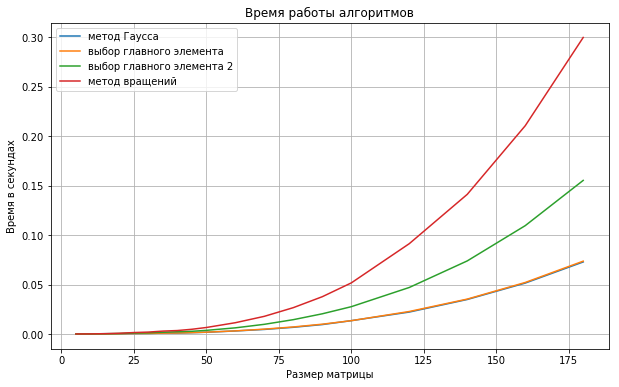
\includegraphics[width=0.9\textwidth]{gr_time.png}

Поскольку время работы всех алгоритмов $O(n^3)$, где $n$ -- размер матрицы, то можно, поделив на $n^3$ результаты измерений, вычислить константу перед старшим членом в времени работы:

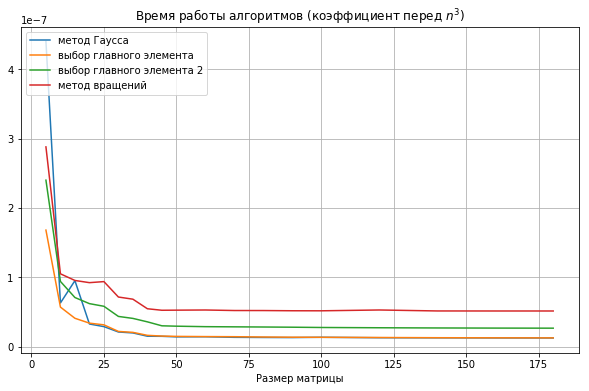
\includegraphics[width=0.9\textwidth]{gr_time_2.png}

\subsection{Точность прямых методов}

Точность оценивалась следующим образом: генерировались вектор $x_0$ и матрица $A$. Вектор $b$ вычислялся как $b = Ax_0$. Далее алгоритм находил решение уравнения $Ax=b$ и считалась относительная погрешность его ответа: $\frac{|x - x_0|}{x_0}$. Здесь используется норма $|| A ||_1 = \max_{j=1}^m \left( \sum_{i=1}^n |A_{ij}| \right)$.

На матрицах из случайных чисел от 0 до 1 точность всех алгоритмов была высокой, поскольку сгенерированные 
таким образом матрицы обладают небольшим числом обусловленности.

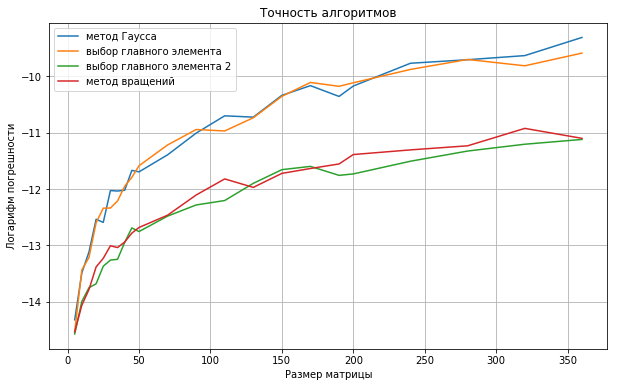
\includegraphics[width=0.9\textwidth]{gr_acc_good.png}

Также была измерена точность на матрицах с высоким числом обусловленности. Для этого генерировались матрицы, близкие к линейно зависимым.
%написать как именно
Как видно из графика, точность на них значительно меньше:

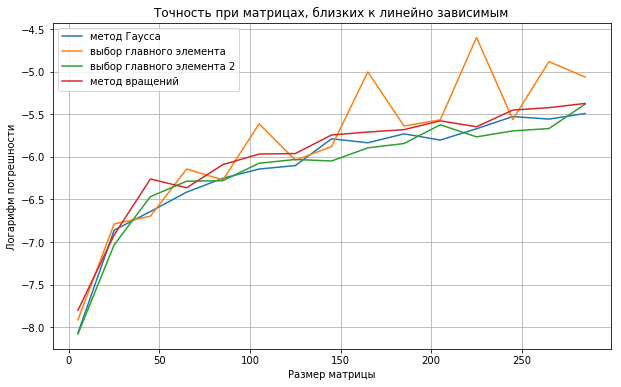
\includegraphics[width=0.9\textwidth]{gr_acc_bad.png}

На матрицах Гильберта (матрицы, в которых $a_{ij} = \frac{1}{i + j - 1}$) точность очень быстро падает с увеличением размерности матриц:

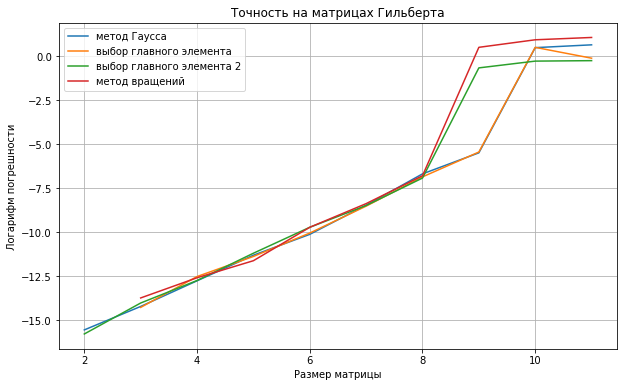
\includegraphics[width=0.6\textwidth]{hilb.png}

\subsection{Итерационные методы}

Для сходимости достаточным условием является то, что $ ||B||_1 < 1$. Поэтому генерировались матрицы с нормой $k<1$ (на графиках ниже 0.6) и к ним прибавлялась единичная матрица. Чтобы сгенерировать матрицу с заданной нормой, бралась матрица $A_0$ из случайных чисел и все её элементы умножались на $\frac{k}{||A||_1}$.

График зависимости точности приближения от количество итераций для двух методов (разные линии соответствуют разным размерам матрицы):

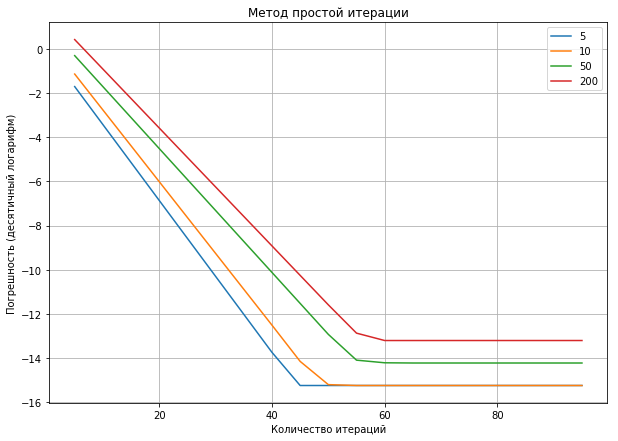
\includegraphics[width=0.7\textwidth]{iter_1.png}

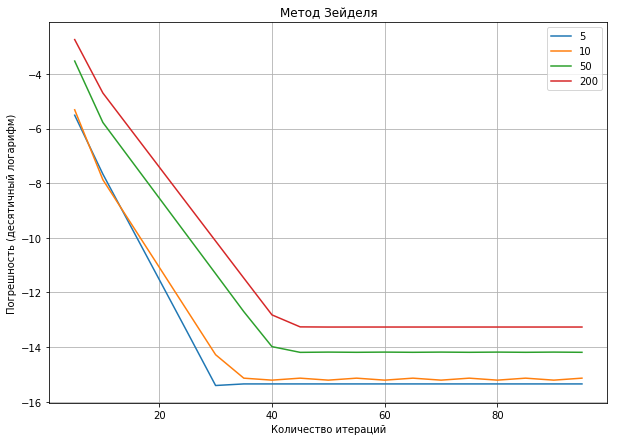
\includegraphics[width=0.7\textwidth]{iter_2.png}

Видно, что отклонение от решения системы убывает экспоненциально (поскольку на графике его логарифм, то график является прямой линией), но с некоторого момента стабилизируется, что связано с точностью вещественных чисел в компьютере. И что метод Зейделя обеспечивает чуть более быструю сходимость.

Однако рассмотрим решение уравнения методом Зейделя $\begin{pmatrix} 1 & 2 \\ 3 & 4 \end{pmatrix} X = \begin{pmatrix} 1 \\ 2 \end{pmatrix}$:

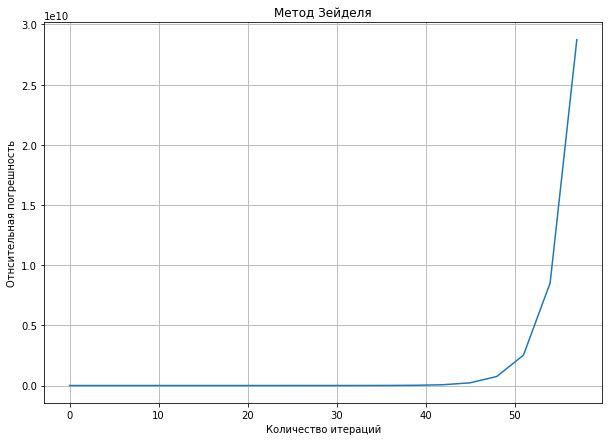
\includegraphics[width=0.6\textwidth]{not_conv.png}

Относительная погрешность возрастает с увеличинием количества операций, процесс не сходится.

\newcommand{\lm}{\lambda}

Действительно, критерий сходимости метода Зейделя: все решения уравнения

$ \det \begin{pmatrix}
\lm a_{11} & a_{12} & \dots & a_{1n} \\
\lm a_{21} & \lm a_{22} & \dots & \dots \\
\dots & \dots & \dots &  \dots \\
\lm a_{n1} & \lm a_{n2} & \dots & \lm a_{nn} \\
\end{pmatrix}$ \\
по модулю должны быть меньше единицы (здесь $a_{ij}$ -- числа из исходной матрицы в уравнении).
Однако в рассмотреном случае суещствует решение $\lm = 1.5$.

\section{Заключение:}
Таким образом, алгоритм Гаусса и алгоритм Гаусса с выбором главного элемента по столбцу обладают примерно одинаковой точностью и временем работы. Алгоритм Гаусса с выбором главного элемента по подматрице медленнее, но обладает большей точностью. Метод вращений ещё медленнее, но обладает примерно одинаковой точностью с выбором главного элемента по подматрице.

Итерационные методы эффективнее, когда количество итераций, необходимое для достижения нужной точности значительно меньше $n$, поскольку время их работы $O(n^2 k)$, где $k$ -- количество итераций, а время работы точных методов $O(n^3)$.

\section{Список использованной литературы:}
\begin{enumerate}
    \item Богачёв К.Ю. Практикум на ЭВМ. Методы решения линейных систем и нахождения собственных значений. -- М.: МГУ им. М.В. Ломоносова, 1998. -- 137 с.
    \item Петров, И. Б. Лекции по вычислительной математике / И.Б. Петров, А.И. Лобанов. -- М.: Интернет-университет информационных технологий, Бином. Лаборатория знаний, 2013. -- 528 c.
\end{enumerate}

\end{document}